% === Einheit  ====================================================================
\Tut\chapter{Quantitative Aspekte von Algorithmen}
\label{k:quantitative-aspekte}
\Tutonly{\begin{center}\Large\bfseries Hinweise f\"ur die Tutorien\end{center}}

% -----------------------------------------------------------------------
\Tut\section{Ressourcenverbrauch bei Berechnungen}
\label{sec:ressourcen}

Wir haben in \hyperref[k:alg-graphen]{Einheit~\ref{k:alg-graphen} mit
  ersten Graphalgorithmen} damit begonnen, festzustellen, wieviele
arithmetische Operationen bei der Ausführung eines Algorithmus für
eine konkrete Probleminstanz ausgeführt werden. Zum Beispiel hatten
wir angemerkt, dass bei der Addition zweier $n\x n$-Matrizen mittels
zweier ineinander geschachtelten \kw{for}-Schleifen $n^2$ Additionen
notwendig sind. Das war auch als ein erster Schritt gedacht in
Richtung der Abschätzung von Laufzeiten von Algorithmen.

\mdefine[Laufzeit, Rechenzeit]{Rechenzeit}\index{Rechenzeit} ist wohl
die am häufigsten untersuchte \mdefine{Ressource}\index{Ressource},
die von Algorithmen "`verbraucht"' wird. Eine zweite ist der
\mdefine{Speicherplatzbedarf}\index{Speicherplatzbedarf}. Man spricht
in diesem Zusammenhang auch von
\mdefine[Komplexitätsmaß]{Komplexitätsmaßen}\index{Komplexitätsmaß}. Sie
sind Untersuchungsgegenstand in Vorlesungen über Komplexitätstheorie
(\engl{computational complexity}\index{computational complexity}) und
tauchen darüber hinaus in vielen Gebieten (und Vorlesungen) zur
Beurteilung der Qualität von Algorithmen auf.

Hauptgegenstand dieser Einheit wird es sein, das wichtigste
Handwerkszeug bereitzustellen, das beim Reden über und beim Ausrechnen
von \zB Laufzeiten hilfreich ist und in der Literatur immer wieder
auftaucht, insbesondere die sogenannte Groß"=O"=Notation.

Dazu sei als erstes noch einmal explizit daran erinnert, dass wir in
\hyperref[k:algorithmusbegriff]{Einheit~\ref{k:algorithmusbegriff} zum
  informellen Algorithmusbegriff} festgehalten haben, dass ein
Algorithmus für Eingaben beliebiger Größe funktionieren sollte: Ein
Algorithmus zur Multiplikation von Matrizen sollte nicht nur für $3\x
3$-Matrizen oder $42\x 42$"=Matrizen funktionieren, sollte für
Matrizen mit beliebiger Größe $n\x n$. Es ist aber "`irgendwie klar"',
dass dann die Laufzeit keine Konstante sein kann, sondern eine
Funktion ist, die zumindest von $n$ abhängt. Und zum Beispiel bei
Algorithmus~\ref{alg:wege-n-hoch-5} zur Bestimmung der Wegematrix
eines Graphen hatte auch nichts anderes als die Größe Einfluss auf die
Laufzeit.

Aber betrachten wir als ein anderes Beispiel das Sortieren von Zahlen
und \zB den Insertionsort-Algorithmus aus der
Programmieren"=Vorlesung, den wir in
Algorithmus~\ref{alg:insertionsort} noch mal aufgeschrieben haben. Wie
oft die \kw{for}"=Schleife in der Methode @v{insert} ausgeführt
wird, hängt nicht einfach von der Problemgröße $n=@v{a.length}$ ab. Es
hängt auch von der konkreten Probleminstanz ab. Selbst bei gleicher
Zahl $n$ kann die Schleife unterschiedlich oft durchlaufen werden: Ist
das Array @v{a} von Anfang an sortiert, wird die \kw{for}"=Schleife
überhaupt nicht ausgeführt. Ist es genau in entgegengesetzter Richtung
sortiert, wird ihr Schleifenrumpf insgesamt $\sum_{i=1}^{n-1}i =
n(n-1)/2$ mal ausgeführt.

% \begin{tutorium}
%   Snelting hat in seiner Vorlesung umgestellt.  Den im Skript
%   zitierten Insertionsort-Algorithmus haben die Studenten in
%   Programmieren bis zum 9.12. wohl noch nicht gesehen. Nicht darauf
%   aufbauen.

%   Im vorgezogenen Abschnitt "`Rekursion"' tauchen aber die
%   Binomialkoeffizienten auf:
%   \[
%   \binom{n}{k}=\begin{cases}
%     0 & \text{ falls } k=0\lor k=n\\
%     \binom{n-1}{k-1}+\binom{n-1}{k} & \text{ sonst}
%   \end{cases}
%   \]
% \end{tutorium}

\begin{algorithm}[h]
  \begin{tabbing}
    \quad\=\quad\=\quad\=\quad\=\quad\=\hspace*{30mm}\=\\[-\baselineskip] \kill
    \kw{public} \kw{class} $@v{InsertionSort}$ \{ \\
    \> \kw{public} \kw{static} \kw{void} $@v{sort}(\kw{long}[\,]\; @v{a})$ \{ \\
      \>\> \kw{for} $(\kw{int}\; @v{i} <- 1; \;\; @v{i} < @v{a}.@v{length};\;\;  @v{i}++)$ \{ \\
        \>\>\> $@v{insert}(@v{a}, @v{i})$; \\
        \>\> \} \\
      \> \} \\
  % \>    \kw{private} \kw{static} \kw{void} $@v{insert}(\kw{long}[\,]\; @v{a}, \kw{int}\; @v{idx})$ \{ \\
  % \>\>       \kw{int} $@v{i} <- @v{idx}$; \\
  % \>\>       /\!\!/ Tausche $@v{a}[@v{idx}]$ nach links bis es einsortiert ist \\
  % \>\>       \kw{while} $(@v{i} > 0 \;\land\; @v{a}[@v{i} - 1] > @v{a}[@v{i}])$ \{ \\
  % \>\>\>         \kw{long} $@v{tmp} <- @v{a}[@v{i} - 1]$; \\
  % \>\>\>         $@v{a}[@v{i} - 1] <- @v{a}[@v{i}]$; \\
  % \>\>\>         $@v{a}[@v{i}] <- @v{tmp}$; \\
  % \>\>\>         $@v{i}- -$; \\
  % \>\>       \} \\
  % \>     \} \\
   \>    \kw{private} \kw{static} \kw{void} $@v{insert}(\kw{long}[\,]\; @v{a}, \kw{int}\; @v{idx})$ \{ \\
   \>\>       /\!\!/ Tausche $@v{a}[@v{idx}]$ nach links bis es einsortiert ist \\
   \>\>       \kw{for} (\kw{int} $@v{i} <- @v{idx}$; $@v{i} > 0$ \kw{and} $@v{a}[@v{i}-1] > @v{a}[@v{i}]$; $@v{i}- -$) \{    \\
   \>\>\>         \kw{long} $@v{tmp} <- @v{a}[@v{i} - 1]$; \\
   \>\>\>         $@v{a}[@v{i} - 1] <- @v{a}[@v{i}]$; \\
   \>\>\>         $@v{a}[@v{i}] <- @v{tmp}$; \\
   \>\>       \} \\

   \>     \} \\
   \} \\[-\baselineskip]
  \end{tabbing}
  \caption{Insertionsort aus der Vorlesung "`Programmieren"'}
  \label{alg:insertionsort}
\end{algorithm}

Meistens ist es aber so, dass man nicht für jede Probleminstanz
einzeln angeben will oder kann, wie lange ein Algorithmus zu seiner
Lösung benötigt. Man beschränkt sich auf eine vergröbernde Sichtweise
und beschreibt \zB die Laufzeit nur in Abhängigkeit von der
Problemgröße $n$. Es bleibt die Frage zu klären, was man dann angibt,
wenn die Laufzeit für verschiedene Instanzen gleicher Größe variiert:
Den Durchschnitt? Den schnellsten Fall? Den langsamsten Fall?

Am weitesten verbreitet ist es, als Funktionswert für jede
Problemgröße $n$ den jeweils schlechtesten Fall (\engl{worst
  case})\graffito{worst case}\index{worst case} zu nehmen.  Eine
entsprechende Analyse eines Algorithmus ist typischerweise deutlich
einfacher als die Berechnung von Mittelwerten (\engl{average
  case})\graffito{average case}\index{average case}, und wir werden
uns jedenfalls in dieser Vorlesung darauf beschränken.

% -----------------------------------------------------------------------
\Tut\section{Gro\ss-O-Notation}
\label{sec:gross-o}

\index{Groß-O-Notation}Die Aufgabe besteht also im allgemeinen darin,
bei einem Algorithmus für jede mögliche Eingabegröße $n$ genau
anzugeben, wie lange der Algorithmus für Probleminstanzen der Größe
$n$ im schlimmsten Fall zur Berechung des Ergebnisses benötigt. Leider
ist es manchmal so, dass man die exakten Werte nicht bestimmen will
oder kann.

Dass man es nicht \emph{will}, muss nicht unbedingt Ausdruck von Faulheit
sein. Vielleicht sind gewisse Ungenauigkeiten (die man noch im Griff
hat) für das Verständnis nicht nötig. Oder die genauen Werte hängen
von Umständen ab, die sich ohnehin "`bald"' ändern. Man denke etwa an
die recht schnelle Entwicklung bei Prozessoren in den vergangenen
Jahren. Dass ein Programm für gewisse Eingaben auf einem bestimmten
Prozessor soundso lange braucht, ist unter Umständen schon nach
wenigen Monaten uninteressant, weil ein neuer Prozessor viel schneller
ist. Das muss nicht einfach an einer höheren Taktrate liegen (man
könnte ja auch einfach Takte zählen statt Nanosekunden), sondern \zB
an Verbesserungen bei der Prozessorarchitektur.

Darüber hinaus \emph{kann} man die Laufzeit eines Algorithmus mitunter
gar nicht exakt abschätzen.  Manchmal könnte man es vielleicht im
Prinzip, aber man ist zu dumm.  Oder die vergröbernde Darstellung nur
der schlechtesten Fälle führt eben dazu, dass die Angabe für andere
Fälle nur eine obere Schranke ist. Oder man erlaubt sich bei der
Formulierung von Algorithmen gewisse Freiheiten \bzw Ungenauigkeiten,
die man (vielleicht wieder je nach Prozessorarchitektur)
unterschiedlich bereinigen kann, weil man eben an Aussagen
interessiert ist, die von Spezifika der Prozessoren unabhängig sind.

Damit haben wir zweierlei angedeutet: 
%
\begin{itemize}
\item Zum einen werden wir im weiteren Verlauf dieses Abschnittes eine
  Formulierungshilfe bereitstellen, die es erlaubt, in einem gewissen
  überschaubaren Rahmen ungenau über Funktionen zu reden.
\item Zum anderen werden wir in einer späteren Einheit auf Modelle für
  Rechner zu sprechen kommen. Ziel wird es sein, \zB über Laufzeit von
  Algorithmen in einer Weise reden zu können, die unabhängig von
  konkreten Ausprägungen von Hardware sind und trotzdem noch
  aussagekräftig ist.
\end{itemize}
%

% -----------------------------------------------------------------------
\Tut\subsection{Ignorieren konstanter Faktoren}
\label{subsec:gross-theta}

\begin{tutorium}
  Wir machen das ein bisschen anders als andere:
  \begin{itemize}
  \item erst wird $\Theta$ eingeführt, und danach $O$: 
    \begin{itemize}
    \item ich finde, dass $\Theta$ das näher liegende ist, und man
      kann sich erst mal drauf beschränken, dass Ignorieren konstanter
      Faktoren kennenzulernen
    \item die Verallgemeinerungen zu $O$ und $\Omega$ sind dann
      leichter (meiner Meinung nach)
    \end{itemize}
  \item ich führe erst eine Äquivalenzrelation $\asymp$ ein, und dann
    $\Theta(f)$ als Äquivalenzklasse (ohne dieses Wort schon zu
    benutzen) von Funktionen.
  \item auch so ist hinterher leicht zu sehen, dass $\Theta(f)=O(f)\cap
    \Omega(f)$.
  \item Achtung: einiges könnte man auch leicht unter Verwendung von
    $\lim$, oder genauer mit $\limsup$ argumentieren, aber ich weiß
    nicht, wie weit die Informationswirte in ihrer Mathematik sind.
  \end{itemize}
\end{tutorium}
Wie ungenau wollen wir über Funktionen reden?

Ein erster Aspekt wird dadurch motiviert, dass man das so tun möchte,
dass \zB Geschwindigkeitssteigerungen bei Prozessoren irrelevant
sind. Etwas genauer gesagt sollen konstante Faktoren beim Wachstum von
Funktionen keine Rolle spielen.

Wir bezeichnen im folgenden mit $\Rplus$ die Menge der positiven reellen
Zahlen (also \emph{ohne} $0$) und mit $\R_0^+$ die Menge der
nichtnegativen rellen Zahlen, also $\R_0^+=\Rplus \cup\{0\}$. Wir
betrachten Funktionen $f:\N_0 ->\R_0^+$.

Wir werden im folgenden vom \mdefine[asymptotisches
Wachstum]{asymptotischen Wachstum}\index{asymptotisches
  Wachstum}\index{Wachstum!asymptotisches} oder auch
\mdefine[größenordnungsmäßiges Wachstum]{größenordnungsmäßigen
  Wachstum}\index{größenordnungsmäßiges
  Wachstum}\index{Wachstum!größenordnungsmäßig} von Funktionen
sprechen (obwohl es das Wort "`größenordnungsmäßig"' im Deutschen gar
nicht gibt --- zumindest steht es nicht im Duden; betrachten wir es
als Terminus technicus). Eine Funktion $g:\N_0 ->\R_0^+$ wächst
\define{größenordnungsmäßig genauso
  schnell}\index{Wachstum!größenordnungsmäßig gleich} wie eine
Funktion $f:\N_0 ->\R_0^+$, wenn gilt:
\[
\exists c,c'\in \Rplus: \exists n_0\in \N_0: \forall n\geq n_0: c f(n)
\leq g(n) \leq c' f(n) \;.
\]
Wir schreiben in diesem Fall auch \mdefine{$f\asymp g$}\index{$f\asymp
g$} oder $f(n)\asymp g(n)$.  Zum Beispiel gilt $3n^2 \asymp 10^{-2}
n^2$. Denn einerseits gilt für $c= 10^{-3}$ und $n_0=0$:
\[
\forall n\geq n_0: c f(n) = 10^{-3}\cdot 3n^2 \leq 10^{-2} n^2 = g(n)
\]
Andererseits gilt \zB für $c'=1$ und $n_0=0$:
\[
\forall n\geq n_0: g(n)=10^{-2} n^2 \leq 3 n^2 = c' f(n)
\]
%
Die eben durchgeführte Rechnung lässt sich leicht etwas allgemeiner
durchführen. Dann zeigt sich, dass man festhalten kann:

\begin{punkt}[Rechenregel]
  \label{rr:a-b-asymp}
  Für alle $f:\N_0 -> \Rnullplus$ gilt:
  \[
  \forall a,b\in\Rplus:  a f(n) \asymp b f(n)
  \]
\end{punkt}
% 
Damit können wir uns als zweites Beispiel $f(n)=n^3+5n^2$ und
$g(n)=3n^3-n$ ansehen und nun schon recht leicht einsehen, dass
$f\asymp g$ ist. Denn einerseits ist für $n\geq 0$ offensichtlich
$f(n)=n^3+5n^2 \leq n^3+5n^3 = 6n^3 = 9n^3-3n^3\leq
9n^3-3n=3(3n^3-n)=3g(n)$. Andererseits ist $g(n) = 3n^3-n \leq 3n^3
\leq 3(n^3+5n^2) = 3f(n)$.

\begin{tutorium}
  $\Theta$ und Polynome: Man versuche klar zu machen, dass immer
  $f\asymp g$ ist, wenn $f$ und $g$ Polynome gleichen Grades sind,
  also \zB $42n^6-33n^3+222n^2 -15 \asymp 66n^6+55555n^5$. Das kann
  man \zB in Anlehnung an $n^3+5n^2\asymp 3n^3-n$ aus der Vorlesung
  machen.
\end{tutorium}

Es gibt auch Funktionen, für die $f\asymp g$ \emph{nicht} gilt. Als
einfaches Beispiel betrachten wir $f(n)=n^2$ und $g(n)=n^3$. Die
Bedingung $g(n) \leq c'f(n)$ aus der Definition ist für $f(n)\not=0$
gleichbedeutend mit $g(n)/f(n) \leq c'$. Damit $f\asymp g$ gilt, muss
insbesondere $g(n)/f(n) \leq c'$ für ein $c'\in \Rplus$ ab einem $n_0$
für alle $n$ gelten. Es ist aber $g(n)/f(n)=n$, und das kann durch
keine Konstante beschränkt werden.

Mitunter ist eine graphische Darstellung nützlich. In
Abbildung~\ref{fig:asymp-1} sieht man zweimal die gleiche Funktion
$f(x)$ für den gleichen Argumentbereich geplottet. Auf der linken
Seite sind beide Achsen linear skaliert. Auf der rechten Seite ist die
$y$-Achse logarithmisch skaliert. In einer solchen Dartstellung erhält
man den Graph für $cf(x)$ aus dem für $f(x)$ durch Verschieben um
$\log(c)$ nach oben.
%
\begin{figure}[ht]
  \centering
  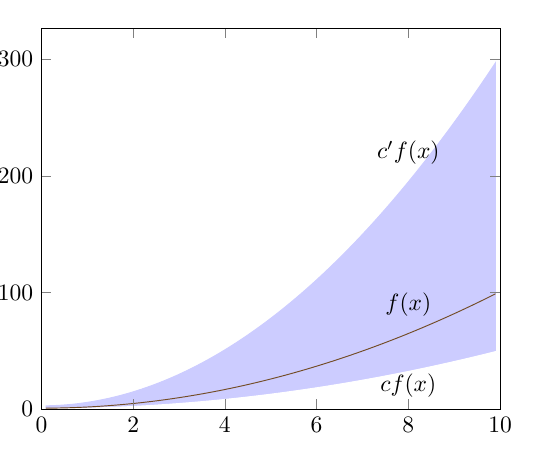
\begin{tikzpicture}[domain=0.1:9.9,samples=100,scale=0.85]
    \begin{axis}[xmin=0,xmax=10,ymin=0.1,
      axis on top,
      % area style,
      ymode=normal,
      ylabel style={overlay},
      yticklabel style={overlay},
      no markers]
      \addplot+[fill,color=blue!20!white] expression {3*(1+x^2)}  \closedcycle;
      \addplot+[fill,color=white] expression {0.5*(1+x^2)}  \closedcycle;
      \addplot expression {1+x^2};
      % \addplot expression {1.2+x*(1+0.4*sin(x*90))};
      \node at (axis cs:8,220) {$c'f(x)$};
      \node at (axis cs:8,90) {$f(x)$};
      \node at (axis cs:8,20) {$cf(x)$};
    \end{axis}
  \end{tikzpicture}
\hspace*{10mm}
  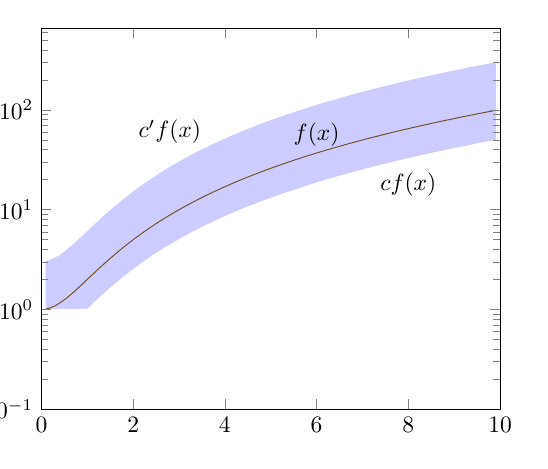
\begin{tikzpicture}[domain=0.1:9.9,samples=100,scale=0.85]
    \begin{axis}[xmin=0,xmax=10,ymin=0.1,
      axis on top,
      % area style,
      ymode=log,
      ylabel style={overlay},
      yticklabel style={overlay},
      no markers]
      \addplot+[fill,color=blue!20!white] expression {3*(1+x^2)}  \closedcycle;
      \addplot+[fill,color=white] expression {0.5*(1+x^2)}  \closedcycle;
      \addplot expression {1+x^2};
      % \addplot expression {1.2+x*(1+0.4*sin(x*90))};
      \node at (axis cs:2.8,60) {$c'f(x)$};
      \node at (axis cs:6,57) {$f(x)$};
      \node at (axis cs:8,18) {$cf(x)$};
    \end{axis}
  \end{tikzpicture}
  %
  \caption{Zweimal die gleiche Funktion $f(x)$ und zwei Schranken
    $cf(x)$ und $c'f(x)$; links Darstellung mit linear skalierter
    $y$-Achse, rechts mit logarithmisch skalierter $y$-Achse}
  \label{fig:asymp-1}
\end{figure}
%
Für eine Funktion $g(x)$ mit $g(x)\asymp f(x)$ muss gelten, dass, von
endlich vielen Ausnahmen abgesehen, für "`fast"' alle $n\in \N_0$
gilt: $c f(n) \leq g(n) \leq c' f(n)$. Auf die graphische Darstellung
übertragen bedeutet das, dass der Graph für $g$ fast überall in dem
farblich hinterlegten "`Schlauch"' um $f$ liegen muss. In
Abbildung~\ref{fig:asymp-2} ist ein Beispiel dargestellt.

\begin{figure}[ht]
  \centering
  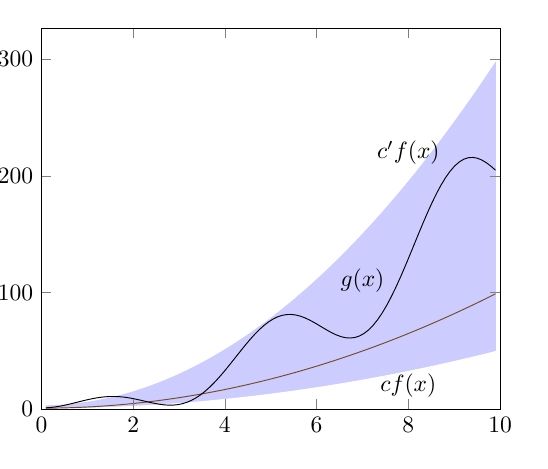
\begin{tikzpicture}[domain=0.1:9.9,samples=100,scale=0.85]
    \begin{axis}[xmin=0,xmax=10,ymin=0.1,
      axis on top,
      % area style,
      ymode=normal,
      ylabel style={overlay},
      yticklabel style={overlay},
      no markers]
      \addplot+[fill,color=blue!20!white] expression {3*(1+x^2)}  \closedcycle;
      \addplot+[fill,color=white] expression {0.5*(1+x^2)}  \closedcycle;
      \addplot expression {1+x^2};
      \addplot expression {1.2+x^2*(2+5*sin(x*90)/x)};
      \node at (axis cs:8,220) {$c'f(x)$};
      \node at (axis cs:8,20) {$cf(x)$};
      \node at (axis cs:7,110) {$g(x)$};
    \end{axis}
  \end{tikzpicture}
\hspace*{10mm}
  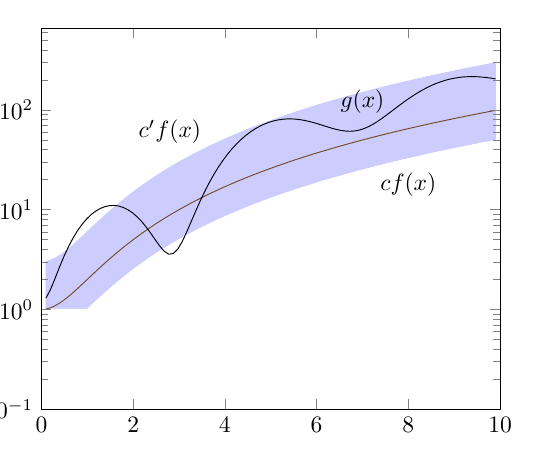
\begin{tikzpicture}[domain=0.1:9.9,samples=100,scale=0.85]
    \begin{axis}[xmin=0,xmax=10,ymin=0.1,
      axis on top,
      % area style,
      ymode=log,
      ylabel style={overlay},
      yticklabel style={overlay},
      no markers]
      \addplot+[fill,color=blue!20!white] expression {3*(1+x^2)}  \closedcycle;
      \addplot+[fill,color=white] expression {0.5*(1+x^2)}  \closedcycle;
      \addplot expression {1+x^2};
      \addplot expression {1.2+x^2*(2+5*sin(x*90)/x)};
      \node at (axis cs:2.8,60) {$c'f(x)$};
      \node at (axis cs:8,18) {$cf(x)$};
      \node at (axis cs:7,120) {$g(x)$};
    \end{axis}
  \end{tikzpicture}
  %
  
  \caption{Zweimal die gleiche Funktion $g(x)$, die für $n\geq 4$ durch
    $c f(n)$ und $c' f(n)$ beschränkt ist.}
  \label{fig:asymp-2}
\end{figure}

Wer mit Grenzwerten schon vertraut ist, dem wird auch klar sein, dass
\zB nicht $n^2 \asymp 2^n$ ist: Da $\lim_{n->oo} 2^n/n^2=oo$ ist, ist
offensichtlich \emph{nicht} für alle großen $n$ die Ungleichung
$2^n\leq c' n^2$ erfüllbar. Man kann sich das aber auch "`zu Fuß"'
überlegen: Für die Folge von Zahlen $n_i=2^{i+2}$ gilt:
\[
\forall i\in\N_0: 2^{n_i} \geq 4^i n_i^2
\]
Der Induktionsanfang ist klar und es ist
\[
  2^{n_{i+1}} = 2^{2n_i} = 2^{n_i} \cdot 2^{n_i} 
  \geq 4^i n_i^2 \cdot 4^{n_i/2} 
  \geq 4^i n_i^2 \cdot 16 
  = 4^i \cdot 4 \cdot 4 n_i^2 = 4^{i+1} \cdot n_{i+1}^2   \;.
\]
Also kann nicht für alle großen $n$ gelten: $2^n \leq c n^2$.

Das Zeichen $\asymp$ erinnert an das Gleichheitszeichen. Das ist auch
bewusst so gemacht, denn die Relation $\asymp$ hat wichtige
Eigenschaften, die auch auf Gleichheit zutreffen:

\begin{lemma}
  Die Relation $\asymp$ ist eine Äquivalenzrelation.
\end{lemma}
% 
\begin{beweis}
  Wir überprüfen die drei definierenden Eigenschaften von
  Äquivalenzrelationen (siehe
  Abschnitt~\ref{subsec:symm-rel-equiv-rel}).
  \begin{itemize}
  \item \emph{Reflexitvität}: Es ist stets $f\asymp f$, denn wenn man
    $c=c'=1$ und $n_0=0$ wählt, dann gilt für $n\geq n_0$ offensichtlich
    $c f(n) \leq f(n) \leq c' f(n)$.
  \item \emph{Symmetrie:} Wenn $f\asymp g$ gilt, dann auch $g\asymp f$:
    Denn wenn für positive Konstanten $c, c'$ und alle $n\geq n_0$ 
    \[
    c f(n) \leq g(n) \leq c' f(n)
    \]
    gilt, dann gilt für die gleichen $n\geq n_0$ und die ebenfalls
    positiven Konstanten $d=1/c$ und $d'=1/c'$:
    \[
    d' g(n) \leq f(n) \leq d g(n)
    \]
  \item \emph{Transitivität:} Wenn $f\asymp g$ ist, und $g\asymp h$,
    dann ist auch $f\asymp h$: Es gelte für Konstanten $c,c'\in\Rplus$ und
    alle $n\geq n_0$
    \[
    c f(n) \leq g(n) \leq c' f(n)
    \]
    und analog für Konstanten $d,d'\in\Rplus$ und alle $n\geq n_1$
    \[
    d g(n) \leq h(n) \leq d' g(n) \;.
    \]
    Dann gilt für alle $n\geq \max(n_0, n_1)$
    \[
    dc f(n) \leq d g(n) \leq h(n) \leq d' g(n) \leq d'c' f(n) \;,
    \]
    wobei auch die Konstanten  $dc$ und $d'c'$ wieder positiv sind.
  \end{itemize}
\end{beweis}
% 
Es ist üblich, für die Menge aller Funktionen, die zu einer gegebenen
Funktion $f(n)$ im Sinne von $\asymp$ äquivalent sind,
$\Theta(f)$\graffito{$\Theta(f)$}\index{Theta@$\Th{f}$} \bzw
$\Theta(f(n))$ zu schreiben. Also:
\begin{align*}
  \Th{f} &= \{ g \mid f \asymp g \} \\
  &= \{ g \mid \exists c,c'\in \Rplus: \exists n_0\in \N_0: \forall  n\geq n_0: c f(n) \leq g(n) \leq c' f(n) \} 
\end{align*}

\begin{tutorium}
  Beispiel: Logarithmenfunktionen haben alle größenordnungsmäßig das
  gleiche Wachstum:
  \begin{itemize}
  \item Logarithmen sind ja wohl definitiv Schulwissen. Trotzdem
    darauf vorbereitet sein, dass Fragen kommen. Also: Für $a\in\Rplus$
    und $n\in\N_+$ ist $\log_a(n)$ die Zahl mit $a^{\log_a(n)} = n$.
    Beachte: $n\geq1$, da $\log 0$ nicht definiert.
  \item Man zeige: $\log_2(n) \in\Th{\log_8(n)}$ \\
    \begin{itemize}
    \item man beginne vielleicht mit Beispielen:
      
      \begin{tabular}{*{6}{>{$}r<{$}}}
        n         & 1 & 8 & 64 & 512 & 4096 \\
        \log_8(n) & 0 & 1 &  2 &   3 &    4 \\
        \log_2(n) & 0 & 3 &  6 &   9 &   12 \\
      \end{tabular}

      da sollte man doch was sehen \dots
    \item dann rechnen: $n = 8^{\log_8 n} = (2^3)^{\log_8(n)} = 2
      ^{3\log_8(n)}$, also gilt für alle $n\geq 1$: $\log_2(n) = 3
      \log_8(n)$ und $\log_8(n)=\frac{1}{3}\log_2(n)$
    \item wenn das klar ist, dann wohl auch \dots
    \end{itemize}
  \item allgemein: $\log_b(n) \in\Th{\log_a(n)}$, denn
    \[
    b^{\log_b(n)} = n = a^{\log_a(n)} = (b^{\log_b(a)})^{\log_a(n)} = b^{\log_b(a) \cdot \log_a(n) }
    \]
    also liefert (Exponentiation ist injektiv) der Vergleich der
    Exponenten (oder anders gesagt: Logarithmieren beider Seiten):
    $\log_b(n) = \log_b(a) \cdot \log_a(n)$ \\
    also für $c'=c=\log_b(a)$ und alle $n\geq 1$ gilt: $c \log_a(n)
    \leq\log_b(n) \leq c' \log_a(n) $
  \item Man kann also einfach $\Th{\log n}$ schreiben, ohne die Basis
    anzugeben, denn sie ist egal.
  \end{itemize}
\end{tutorium}

Aus Rechenregel~\ref{rr:a-b-asymp} wird bei Verwendung von $\Theta$:
\begin{punkt}[Rechenregel]
  \label{rr:a-b-theta}
  Für alle $f:\N_0 -> \Rnullplus$ und alle Konstanten $a,b\in\Rplus$ gilt:
  $\Th{a f} = \Th{b f}$.
\end{punkt}
%
Zum Beispiel ist $\Th{3n^2} = \Th{8n^2}$.

% -----------------------------------------------------------------------
\Tut\subsection{Notation f\"ur obere und untere Schranken des Wachstums}
\label{subsec:gross-O}

In Fällen wie der unbekannten Anzahl von Durchläufen der
\kw{for}-Schleife in der Funktion \textit{insert} in
Algorithmus~\ref{alg:insertionsort} genügt es nicht, wenn man
konstante Faktoren ignorieren kann. Man kennt nur den schlimmsten
Fall: $\sum_{i=1}^{n-1}i= n(n-1)/2$. Dementsprechend ist im
schlimmsten Fall die Laufzeit in $\Th{n^2}$; im allgemeinen kann sie
aber auch kleiner sein. Um das bequem ausdrücken und weiterhin
konstante Faktoren ignorieren zu können, definiert man:
\graffito{$\Oh{f}$, $\Om{f}$}\index{O@{$\Oh{f}$}}\index{O2@{$\Om{f}$}}
%
% \begin{align*}
% \Oh{f(n)} &= \{ g(n) \mid \exists c\in \Rplus:\exists n_0\in\N_0: \forall
% n\geq n_0: g(n) \leq c f(n)\}\\
% \Om{f(n)} &= \{ g(n) \mid \exists c\in \Rplus:\exists n_0\in\N_0: \forall
% n\geq n_0: g(n) \geq c f(n)\} 
% \end{align*}
\begin{align*}
\Oh{f} &= \{ g \mid \exists c\in \Rplus:\exists n_0\in\N_0: \forall
n\geq n_0: g(n) \leq c f(n)\}\\
\Om{f} &= \{ g \mid \exists c\in \Rplus:\exists n_0\in\N_0: \forall
n\geq n_0: g(n) \geq c f(n)\} 
\end{align*}
Man schreibt gelegentlich auch\graffito{$g \preceq f$, $g \succeq f$}
\begin{align*}
  g \preceq f &\text{ falls } g\in\Oh{f} \\
  g \succeq f &\text{ falls } g\in\Om{f} 
\end{align*}
%
und sagt, dass $g$ \define{asymptotisch höchstens so schnell wie} $f$
wächst (falls $g\preceq f$) \bzw dass $g$ \define{asymptotisch
  mindestens so schnell wie} $f$ wächst (falls $g\succeq f$).

Betrachten wir drei Beispiele.
\begin{itemize}
\item Es ist $10^{90} n^7 \in \Oh{10^{-90}n^8}$, denn für $c=10^{180}$ ist
  für alle $n\geq 0$: $10^{90} n^7 \leq c\cdot 10^{-90}n^8$. 

  Dieses Beispiel soll noch einmal deutlich machen, dass man in
  $\Oh{\cdot}$ \usw richtig große Konstanten "`verstecken"' kann. Ob
  ein hypothetischer Algorithmus mit Laufzeit in $\Oh{n^8}$ in der
  Praxis wirklich tauglich ist, hängt durchaus davon ab, ob die
  Konstante $c$ bei der oberen Schranke $cn^8$ eher im Bereich
  $10^{-90}$ oder im Bereich $10^{90}$ ist.
\item Mitunter trifft man auch die Schreibweise
  \mdefine{$\Oh{1}$}\index{O1@$\Oh{1}$} an. Was ist das?  Die Definition
  sagt, dass das alle Funktionen $g$ sind, für die es eine
  Konstante $c\in\Rplus$ gibt und ein $n_0\in\N_0$, so dass für alle
  $n\geq n_0$ gilt:
  \[
  g(n) \leq c \cdot 1 = c
  \]
  Das sind also alle Funktionen, die man durch Konstanten beschränken
  kann. Dazu gehören etwa alle konstanten Funktionen, aber auch
  Funktionen wie $3+\sin$. (So etwas habe ich aber noch nie eine
  Rolle spielen sehen.)
\item Weiter vorne hatten wir benutzt, dass der Quotient $n^2/n$ nicht
  für alle hinreichend großen $n$ durch eine Konstante beschränkt
  werden kann. Also gilt \emph{nicht} $n^2\preceq n$. Andererseits
  gilt (machen Sie sich das bitte kurz klar) $n \preceq n^2$. Die
  Relation $\preceq$ ist also \emph{nicht} symmetrisch.

  Allgemein gilt für positive reelle Konstanten $0<a<b$, dass
  $n^a\preceq n^b$ ist, aber \emph{nicht} $n^b\preceq n^a$. Ebenso ist
  für reelle Konstanten $a$ und $b$, die beide echt größer $1$ sind,
  $n^a \preceq b^n$ aber \emph{nicht} $b^n\preceq n^a$.
\end{itemize}
%
Um vom unterschielichen Wachstum einiger Funktionen einen groben
Eindruck zu bekommen, genügt es, sich eine Tabelle mit einigen
Funktionswerten anzusehen:\\

\begin{tabular}{>{$}l<{$} *{6}{>{$}r<{$}}}
  \toprule
  \log_{2}n & 1 & 2 & 3 &   4 &          5 &      6 \\
  n   &  2 &  4 &   8 &    16 &         32 &     64 \\
  n^2 &  4 & 16 &  64 &   256 &       1024 &   4096 \\
  n^3 &  8 & 64 & 512 &  4096 &      32768 & 262144 \\
  2^n &  4 & 16 & 256 & 65536 & 4294967296 & 18446744073709551616 \\
  \bottomrule
\end{tabular}\\

%
\begin{tutorium}
  zum Thema $\Oh{}$:
  \begin{itemize}
  \item Damit die Studenten ein besseres Gefühl für $\Oh{\cdot}$
    bekommen, bitte noch mal genau $n^a\in O(n^b)$ falls $a\leq b$
    betrachten.
  \item Aber damit da kein falscher Eindruck entsteht: \textbf{Bitte
      beachten:} $\preceq$ und $\succeq$ sind \emph{keine} totalen
    Ordnungen. Es gibt unvergleichbare Funktionen. \ZB
    \begin{align*}
      f &=
      \begin{cases}
        1 & \text{ falls $n$ gerade} \\
        n & \text{ falls $n$ ungerade} \\
      \end{cases} \\
      g &=
      \begin{cases}
        n & \text{ falls $n$ gerade} \\
        1 & \text{ falls $n$ ungerade} \\
      \end{cases} \\
    \end{align*}
    Es gilt \emph{nicht} $g\preceq f$, es gilt \emph{nicht} $f\preceq
    g$ und es gilt erst recht \emph{nicht} $f\asymp g$.

    Und das liegt auch nicht daran, dass die Funktionen so hin und her
    springen; für monoton wachsende Funktionen kann man so etwas auch
    machen; das war mal Übungsaufgabe
  \end{itemize}
\end{tutorium}

\noindent
Man muss nur in der Ungleichung $g(n) \leq c f(n)$ die (positive!)
Konstante $c$ auf die andere Seite bringen und schon kann man sich
davon überzeugen, dass gilt:

\begin{punkt}[Rechenregel]
Für alle Funktionen $f:\N_0->\Rnullplus$ und $g:\N_0->\Rnullplus$  gilt:
\[
g\in\Oh{f} \longleftrightarrow f \in\Om{g}, \text{\quad also\quad} g\preceq f \longleftrightarrow f \succeq g
\]
\end{punkt}
% 
Man kann auch zeigen: 
\begin{align*}
\Th{f} &= \Oh{f} \cap \Om{f} \\
\text{also \qquad} g\asymp f &\longleftrightarrow g\preceq f \land g \succeq f
\end{align*}

\begin{tutorium}
  Zu $\Om{\cdot}$: vielleicht auch ein paar einfache Beispiele: Macht
  es den Studenten Probleme, sich von $n^2\in\Om{\log n}$ zu
  überzeugen?
\end{tutorium}


% -----------------------------------------------------------------------
\Tut\subsection{Die furchtbare Schreibweise}
\label{subsec:O-furchbar}

Damit Sie bei Lektüre von Büchern und Aufsätzen alles verstehen, was
dort mit Hilfe von $\Th{\cdot}$, $\Oh{\cdot}$ und $\Om{\cdot}$
aufgeschrieben steht, müssen wir Ihnen nun leider noch etwas
mitteilen. Man benutzt eine (unserer Meinung nach) sehr unschöne (um
nicht zu sagen irreführende) Variante der eben eingeführten
Notation. Aber weil sie so verbreitet ist, muten wir sie Ihnen zu. Man
schreibt nämlich
%
\begin{align*}
  g = \Oh{f}  &\text{\quad statt\quad }  g \in \Oh{f} \;, \\
  g = \Th{f}  &\text{\quad statt\quad }  g \in \Th{f} \;, \\
  g = \Om{f}  &\text{\quad statt\quad }  g \in \Om{f} \;.
\end{align*}
%
Die Ausdrücke auf der linken Seite sehen zwar aus wie Gleichungen,
\emph{aber es sind keine!} Lassen Sie daher bitte immer \emph{große
  Vorsicht} walten: 
\begin{itemize}
\item Es ist \emph{falsch}, aus $g=\Oh{f_1}$ und
  $g=\Oh{f_2}$ zu folgern, dass $\Oh{f_1}=\Oh{f_2}$ ist.
\item Es ist \emph{falsch}, aus $g_1=\Oh{f}$ und
  $g_2=\Oh{f}$ zu folgern, dass $g_1=g_2$ ist.
\end{itemize}
%
Noch furchtbarer ist, dass manchmal etwas von der Art $\Oh{g}=\Oh{f}$
geschrieben wird, \emph{aber nur die Inklusion $\Oh{g}\subseteq
  \Oh{f}$ gemeint ist.}

Auch Ronald Graham\index{Graham, Ronald}, Donald Knuth\index{Knuth,
  Donald} und Oren Patashnik\index{Patashnik, Oren} sind nicht
begeistert, wie man den Ausführungen auf den Seiten~432 und~433 ihres
Buches \citetitle{Graham_1989_CM_bk} \parencite{Graham_1989_CM_bk}
entnehmen kann. Sie geben vier Gründe an, warum man das doch so macht.
Der erste ist Tradition; der zweite ist Tradition; der dritte ist
Tradition. Der vierte ist, dass die Gefahr, etwas falsch zu machen,
oft eher klein ist. Also dann: toi toi toi. Lassen Sie sich niemals
von etwas wie "`$n^2=\Oh{n^3}$"' irritieren.

\begin{tutorium}
  Bitte Fragen beantworten. ABER: Ich sehe zwar einen Grund so etwas
  lesen zu können, aber keinen Grund diesen Unfug schreibenderweise zu
  üben.
\end{tutorium}

% -----------------------------------------------------------------------
\Tut\subsection{Rechnen im O-Kalk\"ul}
\label{subsec:O-kalkuel}

\begin{tutorium}
  Ich habe Probleme, mich in die Probleme der Studenten
  hineinzuversetzen. Es erscheint mir alles so banal :-(
\end{tutorium}

Ist $g_1 \preceq f_1$ und $g_2 \preceq f_2$, dann ist auch $g_1+g_2
\preceq f_1+f_2$.  Ist umgekehrt $g\preceq f_1+f_2$, dann kann man $g$
in der Form $g=g_1+g_2$ schreiben mit $g_1\preceq f_1$ und $g_2\preceq
f_2$.  Das schreiben wir auch so:
\begin{lemma}
  \label{lem:O+O=O}
  Für alle Funktionen $f_1,f_2:\N_0-> \Rnullplus$ gilt:
  \[
  \Oh{f_1} +\Oh{f_2} = \Oh{f_1+f_2}
  \]
\end{lemma}
%
Dabei muss allerdings erst noch etwas definiert werden: die "`Summe"'
von Mengen (von Funktionen). So etwas nennt man manchmal
\mdefine{Komplexoperationen}\index{Komplexoperationen} und definiert
sie so: Sind $M_1$ und $M_2$ Mengen von Elementen, die man addieren
\bzw multiplizieren kann, dann sei
\begin{align*}
  M_1 + M_2     &= \{g_1 + g_2 \mid g_1\in M_1 \land g_2\in M_2\} \\
  M_1 \cdot M_2 &= \{g_1\cdot g_2 \mid g_1\in M_1 \land g_2\in M_2\}
\end{align*}
%
Für Funktionen sei Addition und Multiplikation (natürlich?)
argumentweise definiert. Dann ist \zB
\[
\Oh{n^3}+\Oh{n^3} = \{g_1+ g_2 \mid g_1\in \Oh{n^3} \land g_2\in
\Oh{n^3}\}
\]
\zB
\[
  (2n^3-n^2) + 7n^2 = 2n^3+6n^2 \in\Oh{n^3}+\Oh{n^3}
\]
Wenn eine der Mengen $M_i$ einelementig ist, lässt man manchmal die
Mengenklammern darum weg und schreibt zum Beispiel bei Zahlenmengen
\[
\text{statt \qquad} \{3\}\cdot \N_0+\{1\} \text{\qquad kürzer\qquad} 3\N_0+1
\]
oder bei Funktionenmengen
\[
\text{statt \qquad} \{n^3\}+\Oh{n^2} \text{\qquad kürzer\qquad} n^3+\Oh{n^2} 
\]
Solche Komplexoperationen sind übrigens nichts Neues für Sie. Die
Definition des Produkts formaler Sprachen passt genau in dieses Schema
(siehe Unterabschnitt~\ref{subsec:produkt-sprachen}).

\begin{beweis}[von Lemma~\ref{lem:O+O=O}]
  Wir beweisen die beiden Inklusionen getrennt.
  \begin{description}
  \item["`$\subseteq$"':] Wenn $g_1\in\Oh{f_1}$, dann existiert ein
    $c_1\in\Rplus$ und ein $n_{01}$, so dass für alle $n\geq n_{01}$ gilt:
    $g_1(n) \leq c_1 f_1(n)$. Und wenn $g_2\in\Oh{f_2}$, dann existiert ein
    $c_2\in\Rplus$ und ein $n_{02}$, so dass für alle $n\geq n_{02}$ gilt:
    $g_2(n) \leq c_2 f_2(n)$. 

    Folglich gilt für alle $n\geq n_0=\max(n_{01}, n_{02})$ und für
    $c=\max(c_1,c_2)\in\Rnullplus$:
    \begin{align*}
      g_1(n) + g_2(n) &\leq c_1 f_1(n) + c_2 f_2(n) \\
      &\leq c f_1(n) + c f_2(n) \\
      &= c(f_1(n) + f_2(n))
    \end{align*}
  \item["`$\supseteq$"':] Wenn $g\in\Oh{f_1+f_2}$ ist, dann gibt es
    $c\in\Rplus$ und ein $n_0$, so dass für alle $n\geq n_0$ gilt:
    $g(n)\leq c (f_1(n)+f_2(n))$.

    Man definiere nun eine Funktion $g_1:\N_0->\Rnullplus$ vermöge
    \[
    g_1(n) =
    \begin{cases}
      g(n) & \text{ falls } g(n) \leq cf_1(n) \\
      cf_1(n) & \text{ falls } g(n) > cf_1(n)
    \end{cases}
    \]
    Dann ist offensichtlich $g_1 \in\Oh{f_1}$. 

    Außerdem ist $g_1 \leq g$ und folglich $g_2=g -g_1$
    stets größer gleich $0$. Behauptung: $g_2\in\Oh{f_2}$. Sei $n\geq
    n_0$. Dann ist
    \begin{align*}
      g_2(n) &= g(n) -g_1(n) \\
      &=
      \begin{cases}
        0 & \text{ falls } g(n) \leq cf_1(n)\\
        g(n)-cf_1(n) & \text{ falls } g(n) > cf_1(n)
      \end{cases}\\
      &\leq
      \begin{cases}
        0 & \text{ falls } g(n) \leq cf_1(n)\\
        c (f_1(n)+f_2(n))-cf_1(n) & \text{ falls } g(n) > cf_1(n)
      \end{cases}\\ 
      &=
      \begin{cases}
        0 & \text{ falls } g(n) \leq cf_1(n)\\
        cf_2(n) & \text{ falls } g(n) > cf_1(n)
      \end{cases}\\ 
      &\leq cf_2(n) \;,
    \end{align*}
    also $g_2\in\Oh{f_2}$. Also ist $g=g_1+g_2\in\Oh{f_1}+\Oh{f_2}$.
  \end{description}
\end{beweis}
%
\begin{punkt}[Rechenregel]
  Wenn $g_1\preceq f_1$ ist, und wenn $g_1\asymp g_2$ und $f_1\asymp
  f_2$, dann gilt auch $g_2\preceq f_2$.
\end{punkt}

\begin{punkt}[Rechenregel]
  Wenn $g\preceq f$ ist, also $g\in\Oh{f}$, dann ist auch
  $\Oh{g}\subseteq \Oh{f}$ und $\Oh{g+f}=\Oh{f}$.
\end{punkt}
%
Es gibt noch eine Reihe weiterer Rechenregeln für $\Oh{\cdot}$ und
außerdem ähnliche für $\Th{\cdot}$ und $\Om{\cdot}$ (zum Beispiel
Analoga zu Lemma~\ref{lem:O+O=O}). Wir verzichten hier darauf, sie
alle aufzuzählen.

% -----------------------------------------------------------------------
\Tut\section{Matrixmultiplikation}
\label{sec:matmult}

\def\Nadd{N_{\mathit{add}}}
\def\Nmult{N_{\mathit{mult}}}

Wir wollen uns nun noch einmal ein bisschen genauer mit der
Multiplikation von $n\times n$"=Matrizen beschäftigen, und uns dabei
insbesondere für
\begin{itemize}
\item die Anzahl $\Nadd$ elementarer Additionen ist und
\item die Anzahl $\Nmult$ elementarer Multiplikationen
\end{itemize}
%
interessieren. Deren Summe bestimmt im wesentlichen (\dh bis auf
konstante Faktoren) die Laufzeit.

% -----------------------------------------------------------------------
\Tut\subsection{R\"uckblick auf die Schulmethode}
\label{subsec:matmult-schulmethode}

Die "`Schulmethode"' für die Multiplikation von $2\times 2$"=Matrizen
geht so:
\[
\begin{array}{cc|cc}
  & & b_{11} & b_{12} \\
  & & b_{21} & b_{22} \\ \hline
  a_{11} & a_{12} & a_{11}b_{11} + a_{12}b_{21}& a_{11}b_{12} + a_{12}b_{22}\\
  a_{21} & a_{22} & a_{21}b_{11} + a_{22}b_{21}& a_{21}b_{12} + a_{22}b_{22} \\
\end{array}
\]
%
Wie man sieht ist dabei
\begin{itemize}
\item $\Nmult(2) = 2^2 \cdot 2 = 8$ und
\item $\Nadd(2) = 2^2\cdot(2-1) = 4$.
\end{itemize}
%
Wenn $n$ gerade ist (auf diesen Fall wollen uns im folgenden der
einfacheren Argumentation wegen beschränken), dann ist die
Schulmethode für $n\times n$ Matrizen äquivalent zum Fall, dass man
$2\times2$ Blockmatrizen mit Blöcken der Größe $n/2$ vorliegen hat,
die man nach dem gleichen Schema wie oben multiplizieren kann:
\[
\begin{array}{cc|cc}
  & & B_{11} & B_{12} \\
  & & B_{21} & B_{22} \\ \hline
  A_{11} & A_{12} & A_{11}B_{11} + A_{12}B_{21}& A_{11}B_{12} + A_{12}B_{22}\\
  A_{21} & A_{22} & A_{21}B_{11} + A_{22}B_{21}& A_{21}B_{12} + A_{22}B_{22} \\
\end{array}
\]
%
\begin{tutorium}
  Matrixmultiplikation mit den Blockmatrizen: 
  \begin{itemize}
  \item ich werde das auführlicher erläutern als vergangenes Jahr
  \item trotzdem: vielleicht muss man das noch ein bisschen
    erklären. Man nehme einfach $4\x 4$-Matrizen und sehe sich \zB
    $c_{11}=a_{11}b_{11} + a_{12}b_{21} + a_{13}b_{31} +
    a_{14}b_{41}$:

    Man schreibe sich einige der Blöcke $A_{11}$ \usw hin. Dann sieht
    man: Der erste Teil $a_{11}b_{11} + a_{12}b_{21}$ "`kommt
    von"'/"`passt zu"' $A_{11}B_{11}$ und der zweite Teil
    $a_{13}b_{31} + a_{14}b_{41}$ "`kommt von"'/"`passt zu"'
    $A_{12}B_{21}$.
  \end{itemize}
\end{tutorium}
Das sind $4$ Additionen von Blockmatrizen und $8$ Multiplikationen von
Blockmatrizen. Die Anzahl
elementarer Operationen ist also
\begin{itemize}
\item $\Nmult = 8 \cdot\Nmult(n/2)$ und
\item $\Nadd = 8 \cdot\Nadd(n/2) + 4\cdot (n/2)^2 = 8
  \cdot\Nadd(n/2) + n^2$.
\end{itemize}
%
Wir betrachten den Fall $n=2^k$ (die anderen Fälle gehen im Prinzip
ähnlich). Dann ergibt sich aus $\Nmult = 8 \cdot\Nmult(n/2)$:
\begin{align*}
  \Nmult(2^k) &= 8 \cdot\Nmult(2^{k-1}) = 8 \cdot 8 \cdot\Nmult(2^{k-2}) = \cdots = 8^k \cdot\Nmult(1) \\
  &= 8^k = 8^{\log_2} = 2^{3\log_2} = 2^{\log_2\cdot 3} = n^3
\end{align*}
%
Dass man statt der Pünktchen einen Induktionsbeweis führen kann, ist
Ihnen inzwischen klar, richtig?

Aus $\Nadd = 8 \cdot\Nadd(n/2)+n^2$ ergibt sich analog:
\begin{align*}
  \Nadd(2^k) &= 8 \cdot\Nadd(2^{k-1}) + 4^k \\
  &= 8 \cdot 8 \cdot\Nadd(2^{k-2}) + 8\cdot 4^{k-1} + 4^k= \cdots \\
  &= 8 \cdot 8 \cdot\Nadd(2^{k-2}) + 2\cdot 4^k + 4^k= \cdots \\
  &= 8^k \Nadd(2^0) + (2^{k-1}+ \cdots 1)\cdot 4^k =  \\
  &= 2^k\cdot 4^k \cdot 0 + (2^k -1) \cdot 4^k  =  \\
  &= 2^k\cdot 4^k - 4^k = n^3-n^2
\end{align*}

% -----------------------------------------------------------------------
\Tut\subsection{Algorithmus von Strassen}
\label{subsec:strassen}

\begin{tutorium}
  Ich drücke mich darum, eine rekursive Prozedur hinzuschreiben.

  Immerhin sollte Rekursion in Programmieren dran gewesen sein. Aber wenn
  man das zum ersten Mal hört \dots
\end{tutorium}
%
Nun kommen wir zu der Idee von
\textcite{Strassen_1969_GEO_ar}\index{Strassen, Volker}. Er hat
bemerkt, dass man die Blockmatrizen $C_{ij}$ des Matrixproduktes auch
wie folgt berechnen kann:
\begin{align*}
  M_{1} &=  (A_{11} + A_{22}) (B_{11} + B_{22}) \\
  M_{2} &=  (A_{21} + A_{22}) B_{11} \\
  M_{3} &=  A_{11} (B_{12} - B_{22}) \\
  M_{4} &=  A_{22} (B_{21} - B_{11}) \\
  M_{5} &=  (A_{11} + A_{12}) B_{22} \\
  M_{6} &=  (A_{21} - A_{11}) (B_{11} + B_{12}) \\
  M_{7} &=  (A_{12} - A_{22}) (B_{21} + B_{22}) \\
\noalign{und dann}
  C_{11} &= M_{1} + M_{4} - M_{5} + M_{7} \\
  C_{12} &= M_{3} + M_{5} \\
  C_{21} &= M_{2} + M_{4} \\
  C_{22} &= M_{1} - M_{2} + M_{3} + M_{6}
\end{align*}
%
Das sieht erst einmal umständlicher aus, denn es sind $18$ Additionen
von Blockmatrizen statt nur $4$ bei der Schulmethode.  Aber es sind
nur $7$ Multiplikationen von Blockmatrizen statt $8$! Und das zahlt
sich aus, denn im Gegensatz zum skalaren Fall sind Multiplikationen
aufwändiger als Additionen. Für die Anzahl elementarer Operationen
ergibt sich:
\begin{itemize}
\item $\Nmult = 7 \cdot\Nmult(n/2)$
\item $\Nadd = 7 \cdot\Nadd(n/2) + 18\cdot (n/2)^2 = 7
  \cdot\Nadd(n/2) + 4.5\cdot n^2 $
\end{itemize}
%
Für den Fall $n=2^k$ ergibt sich:
%
\begin{align*}
  \Nmult(2^k) &= 7 \cdot\Nmult(2^{k-1}) = 7 \cdot 7 \cdot\Nmult(2^{k-2}) = \cdots = 7^k \cdot\Nmult(1) \\
  &= 7^k = 7^{\log_2} = 2^{\log_2 7 \cdot \log_2} = n^{\log_2 7} \approx n^{2.807\dots}
\end{align*}
%
Analog erhält man auch für die Anzahl der Additionen $\Nadd
\in\Theta(n^{\log_2 7})$.  Die Gesamtzahl elementarer arithmetischer
Operationen ist also in $\Theta(n^{\log_2 7})+\Theta(n^{\log_2 7})=
\Theta(n^{\log_2 7})\approx\Theta(n^{2.807\dots})$.

Es gibt sogar Algorithmen, die asymptotisch noch weniger Operationen
benötigen. Das in dieser Hinsicht beste Ergebnis war lange Zeit die
Methode von \textcite{Coppersmith_1990_MMA_ar}\index{Coppersmith,
  Don}\index{Winograd, Shmuel}, die mit $\Oh{n^{2.376\dots}}$
elementaren arithmetischen Operationen auskommen. Auch dieses
Verfahren benutzt wie das von Strassen eine Vorgehensweise, die man in
vielen Algorithmen wiederfindet: Man teilt die Probleminstanz in
kleinere Teile auf, die man wie man sagt rekursiv nach dem gleichen
Verfahren bearbeitet und die Teilergebnisse dann benutzt, um das
Resultat für die ursprüngliche Eingabe zu berechnen. Man spricht von
\emph{"`teile und herrsche"'} (\engl{divide and conquer}). Die
aktuelle Rekordhalterin für asymptotisch schnelle Matrixmultiplikation
ist \textcite{Vassilevska_2012_MMF_ip}.


\begin{tutorium}
  Weitere Übungsmöglichkeit: Codeschnipsel aus Sneltings Folien von
  2008 für Berechnung der Binomialkoeffizienten:
\begin{verbatim}
  static int binom(int n, int k) {
    assert n >= k && k >= 0;
    if (k == 0 || k == n) {
      return 1;
    } else {
      return binom(n - 1, k - 1) + binom(n - 1, k);
    }
  }
\end{verbatim}
  Sinz hat in 2012 auch noch eine verbesserte Version mit Cache, die
  wir hier gerade \emph{nicht} betrachten.
  (Seite 29 von \url{http://baldur.ira.uka.de/programmieren-ws1213/Foliensatz_10.pdf})

  Diskussion: Wieviele Aufrufe von \verb|binom| in Abhängigkeit von
  $n$ werden bei der Berechnung eines $\binom{n}{k}$ gemacht? Im
  Detail ist das nicht ganz schön zu machen. Man überzeuge sich aber
  (mit Hilfe eines Beispiels?) davon, dass man mindestens $2^k$ Aufrufe
  der Form $binom(n-k,x)$ mit $0\leq x\leq k$ hat. Das sind im Fall
  $k=n/2$ also immerhin $\left(\sqrt{2}\right)^n$.

  \textbf{Wintersemester 2014/2015}: Auf dem Aufgabenblatt vom 7.1.15
  wird eine Aufgabe zu Binomialkoeffizienten sein. Bitte beachten und
  im Tutorium nicht Lösungen für Teilaufgaben verraten.
\end{tutorium}

% -----------------------------------------------------------------------
\Tut\section{Asymptotisches Verhalten "`implizit"' definierter Funktionen}
\label{sec:master-theorem}

\begin{tutorium}
  Zum Mastertheorem komme ich schätzungsweise erst am 14.1.15. Wenn
  dann in Programmieren rekursives Suchen/Sortieren dran war, gibt es
  mehr Motivation für
  \[
  T = a T\left(\frac{n}{b}\right) + f 
  \] 
\end{tutorium}

Sie werden im Laufe der kommenden Semester viele Algorithmen
kennenlernen, bei denen wie bei Strassens Algorithmus für
Matrixmultiplikation das Prinzip "`Teile und Herrsche"' benutzt
wird. In den einfacheren Fällen muss man zur Bearbeitung eines
Problems der Größe $n$ eine konstante Anzahl $a$ von Teilprobleme
gleicher Größe $n/b$ lösen. Die zusätzlichen Kosten zur Berechnung des
eigentlichen Ergebnisses mögen zusätzlich einen Aufwand $f$
kosten. Das beinhaltet auch den unter Umständen erforderlichen Aufwand
zum Erzeugen der Teilprobleme.

Dann ergibt sich für Abschätzung (\zB) der Laufzeit $T$ eine
Rekursionsformel, die grob gesagt von der Form
\[
T = a T\left(\frac{n}{b}\right) + f 
\] 
ist.  Dabei ist sinnvollerweise $a\geq 1$ und $b>1$. 

Obige Rekursionsformel ist unpräzise, denn Problemgrößen sind immer
ganzzahlig, $n/b$ im allgemeinen aber nicht.  Es zeigt sich aber, dass
sich jedenfalls in den nachfolgend aufgeführten Fällen diese
Ungenauigkeit im folgenden Sinne nicht auswirkt: Wenn man in der
Rekursionsformel $n/b$ durch $\lfloor n/b\rfloor$ oder durch $\lceil
n/b\rceil$ ersetzt oder gar durch $\lfloor n/b+c\rfloor$ oder durch
$\lceil n/b+c\rceil$ für eine Konstante $c$, dann behalten die
folgenden Aussagen ihre Gültigkeit.

Wenn zwischen den Konstanten $a$ und $b$ und der Funktion $f$
gewisse Zusammenhänge bestehen, dann kann man ohne viel Rechnen (das
schon mal jemand anders für uns erledigt hat) eine Aussage darüber
machen, wie stark $T$ wächst.

Es gibt drei wichtige Fälle, in denen jeweils die Zahl $\log_b a$ eine
Rolle spielt:
\begin{description}
\item[Fall 1:] Wenn $f \in \Oh{n^{\log_b a -\eps}}$ für ein
  $\eps>0$ ist, dann ist $T\in \Th{n^{\log_b a}}$.
\item[Fall 2:] Wenn $f \in \Th{n^{\log_b a}}$ ist, dann ist
  $T\in \Th{n^{\log_b a}\log n}$.
\item[Fall 3:] Wenn $f \in \Om{n^{\log_b a +\eps}}$ für ein
  $\eps>0$ ist, und wenn es eine Konstante $d$ gibt mit $0<d<1$, so
  dass für alle hinreichend großen $n$ gilt $af(n/b)\leq d f$, dann
  ist $T\in \Th{f}$.
\end{description}
%
Dass die Aussagen in diesen drei Fällen richtig sind, bezeichnet man
manchmal als \mdefine{Mastertheorem}\index{Mastertheorem}, obwohl es
sich sicherlich um keine sehr tiefschürfenden Erkenntnisse handelt.

Betrachten wir als Beispiele noch einmal die Matrixmultiplikation. Als
"`Problemgröße"' $n$ benutzen wir die Zeilen- \bzw Spaltenzahl.  Der
Fall von $n\x n$-Matrizen wird auf den kleineren Fall von $n/2 \x
n/2$-Matrizen zurückgeführt; es ist also $b=2$.

Bei der Schulmethode haben wir $a=8$ Multiplikationen kleinerer
Matrizen der Größe $n/2$ durchzuführen. In diesem
Fall ist $\log_b a=\log_2 8 = 3$.  Der zusätzliche Aufwand besteht in
$4$ kleinen Matrixadditionen, so dass $f=4\cdot n^2/4=n^2$.  Damit
ist $f\in \Oh{n^{3-\eps}}$ (\zB für $\eps=1/2$) und der erste Fall
des Mastertheorems besagt, dass folglich $T\in\Th{n^3}$. (Und das
hatten wir uns weiter vorne tatsächlich auch klar gemacht.)

Bei Strassens geschickterer Methode sind nur $a=7$ Multiplikationen
kleinerer Matrizen der Größe $n/2$ durchzuführen (es ist wieder
$b=2$). In diesem Fall ist $\log_b a=\log_2 7 \approx 2.807\dots$. Der
zusätzliche Aufwand besteht in $18$ kleinen Matrixadditionen, so dass
$f=18\cdot n^2/4\in \Th{n^2}$. Auch hier gilt für ein geeignetes
$\eps$ wieder $f\in \Oh{n^{\log_b a -\eps}} = \Oh{n^{\log_2
7-\eps}}$. Folglich benötigt Strassens Algorithmus
$T\in\Th{n^{\log_2 7}}= \Th{n^{2.807\dots}}$ Zeit.

\begin{tutorium}
  Mastertheorem
  \begin{itemize}
  \item Fall 2: $f \in \Th{n^{\log_b a}}$ schlägt bei Quicksort zu
    \begin{itemize}
    \item Formel anwenden liefert $n\log n$
    \item schönes Bildchen hilft 
    \end{itemize}
  \item Fall 3: nur bei Nachfragen diskutieren \dots
  \item statt dessen darauf hinweisen, dass einem das Mastertheorem
    nicht weiterhilft, wenn man eine Probleminstanz anders zerhackt,
    wie etwa bei  $(n+1)!=(n+1)*n!$ oder 
    \[
    \binom{n}{k}=\begin{cases}
      0 & \text{ falls } k=0\lor k=n\\
      \binom{n-1}{k-1}+\binom{n-1}{k} & \text{ sonst}
    \end{cases}
    \]
    (siehe weiter vorne)
  \end{itemize}
\end{tutorium}

% -----------------------------------------------------------------------
\Tut\section{Unterschiedliches Wachstum einiger Funktionen}
\label{sec:wachstum-funktionen}

Wir hatten schon darauf hingewiesen, dass gilt:
\begin{enumerate}
\item Für positive reelle Konstanten $0<a<b$ ist $n^a\preceq n^b$,
  aber \emph{nicht} $n^b\preceq n^a$.
\item Für reelle Konstanten $a$ und $b$, die beide echt größer $1$
  sind, gilt $n^a \preceq b^n$ aber \emph{nicht} $b^n\preceq n^a$.
\end{enumerate}
%
Zur Veranschaulichung des ersten Punktes sind in
Abbildung~\ref{fig:wachstum-polynome} die Funktionen $f(x)=x$,
$f(x)=x^2$ und $f(x)=x^3$ geplottet. Allerdings fällt in der gewählten
Darstellung $f(x)=x$ nahezu mit der $x$-Achse zusammen. Wie man sieht,
wird in doppelt-logarithmischen Plots jede Funktion $x^d$ durch eine
Gerade repräsentiert (deren Steigung $d$ ist, wenn die "`Einheiten"'
auf beiden Achsen gleich sind). Allgemeine Polynomfunktionen werden
durch Linien repräsentiert, die sich für große $n$ einer Geraden
anschmiegen.

\begin{figure}[ht]
  \centering
  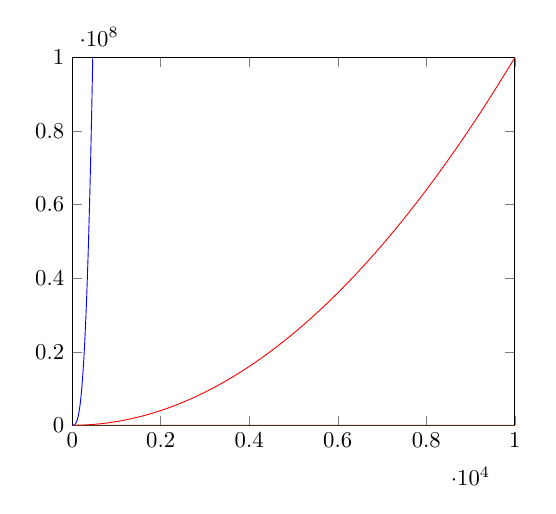
\begin{tikzpicture}[samples=100,scale=0.82,baseline]
    \begin{axis}[xmin=0.9,xmax=10000.0,ymin=0.9,ymax=1e8,no markers
      %,ytickten={0,1,2,3,4}
      ]
      \addplot plot[domain=1:999] expression {x^3};
      \addplot plot[domain=1:9999] expression {x^2};
      \addplot plot[domain=1:9999] expression {x};
    \end{axis}
  \end{tikzpicture}
  %
  \hspace{5mm}
  %
  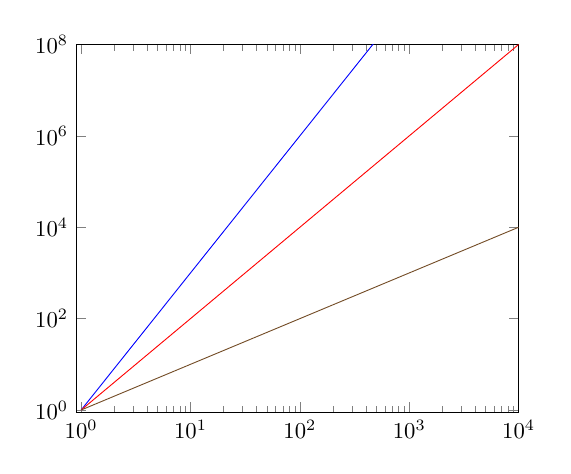
\begin{tikzpicture}[samples=100,scale=0.82,baseline]
    \begin{axis}[xmin=0.9,xmax=10000.0,ymin=0.9,ymax=1e8,no markers
      ,ymode=log,xmode=log
      %,ytickten={0,1,2,3,4}
      ]
      \addplot plot[domain=1:999] expression {x^3};
      \addplot plot[domain=1:9999] expression {x^2};
      \addplot plot[domain=1:9999] expression {x};
    \end{axis}
  \end{tikzpicture}

  \caption{Die Funktionen $f(x)=x$, $f(x)=x^2$ und $f(x)=x^3$ in Plots
    mit linear skalierten Achsen (links) und in doppelt
    logarithmischer Darstellung (rechts); auf der linken Seite ist
    $f(x)=x$ praktisch nicht von der $x$-Achse zu unterscheiden.}
\label{fig:wachstum-polynome}
\end{figure}

Abbildung~\ref{fig:wachstum-exp} zeigt in doppelt-logarithmischer
Darstellung zum Vergleich zwei Polynom- und zwei
Exponentialfunktionen. Der Unterschied sollte klar sein.

\begin{figure}[ht]
  \centering
  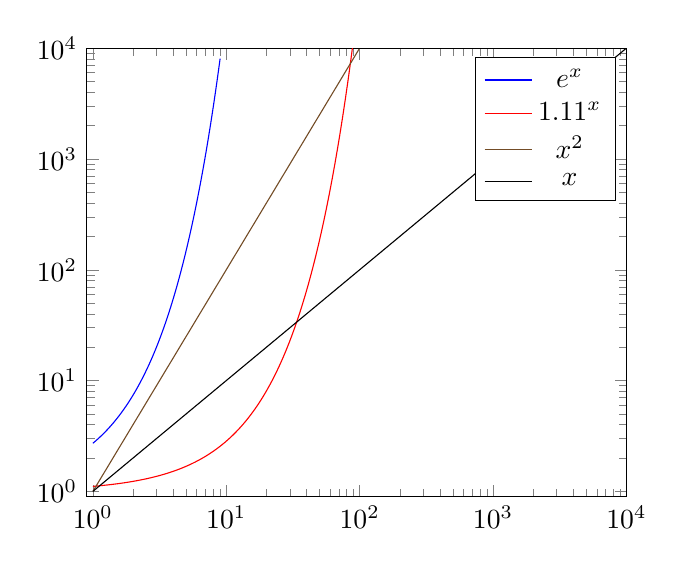
\begin{tikzpicture}[samples=100,scale=1]
    \begin{axis}[xmin=0.9,xmax=10000.0,ymin=0.9,ymax=10000,no markers
      ,ytickten={0,1,2,3,4},ymode=log,xmode=log
      ]
      \addplot plot[domain=1:9] expression {e^x};
      \addlegendentry{$e^x$}
      \addplot plot[domain=1:99] expression {1.11^x};
      \addlegendentry{$1.11^x$}
      \addplot plot[domain=1:99] expression {x^2};
      \addlegendentry{$x^2$}
      \addplot plot[domain=1:9999] expression {x};
      \addlegendentry{$x$}
    \end{axis}
  \end{tikzpicture}

  \caption{Zwei Polynom- und zwei Exponentialfunktionen im Vergleich;
    doppelt-logarithmische Darstellung.}
  \label{fig:wachstum-exp}
\end{figure}

% -----------------------------------------------------------------------
\section{Ausblick}

Algorithmen, bei denen die anderen beiden Fälle des Mastertheorems zum
Tragen kommen, werden Sie im kommenden Semester in der Vorlesung
"`Algorithmen 1"' kennenlernen. 

Manchmal wird "`Teile und Herrsche"' auch in etwas komplizierterer
Form angewendet (zum Beispiel mit deutlich unterschiedlich großen
Teilproblemen). Für solche Situationen gibt Verallgemeinerungen obiger
Aussagen (Satz von Akra und Bazzi).

% -----------------------------------------------------------------------
%  Literatur
% nothing cited in this unit
\printunitbibliography

\cleardoublepage

% -----------------------------------------------------------------------
%%% 
%%% Local Variables:
%%% fill-column: 70
%%% mode: latex
%%% TeX-master: "../k-17-quantitative-aspekte/skript.tex"
%%% TeX-command-default: "XPDFLaTeX"
%%% End:
